\documentclass[11pt]{article}

\usepackage[top=1in,bottom=1in,left=1in,right=1in]{geometry}
\usepackage{amssymb}
\usepackage{amsmath}
\usepackage{graphicx}
\usepackage{setspace}
\usepackage{hyperref}
\usepackage{endnotes}
\usepackage{geometry}
\usepackage{pdflscape}
%\usepackage{pdfpages}
%\usepackage[left=1.25in,right=1.25in]{geometry}

\title{
  \sc
  What Makes a Country Wealthier? \\
  {\large Exploring the determinants of GDP per capita}
}

\author{
    {\rm Kevin Chen '15} \\ 
    \and
    {\rm Varun Sharma '16} \\ 
    \and
    {\rm Jean-Luc Etienne '15} \\ 
}

\hypersetup{
    bookmarks=true,         % show bookmarks bar?
    unicode=false,          % non-Latin characters in Acrobat’s bookmarks
    pdftoolbar=true,        % show Acrobat’s toolbar?
    pdfmenubar=true,        % show Acrobat’s menu?
    pdffitwindow=false,     % window fit to page when opened
    pdfstartview={FitH},    % fits the width of the page to the window
    pdftitle={My title},    % title
    pdfauthor={Author},     % author
    pdfsubject={Subject},   % subject of the document
    pdfcreator={Creator},   % creator of the document
    pdfproducer={Producer}, % producer of the document
    pdfkeywords={keyword1} {key2} {key3}, % list of keywords
    pdfnewwindow=true,      % links in new window
    colorlinks=true,       % false: boxed links; true: colored links
    linkcolor=red,          % color of internal links (change box color with linkbordercolor)
    citecolor=green,        % color of links to bibliography
    filecolor=magenta,      % color of file links
    urlcolor=cyan           % color of external links
}

\begin{document}

\date{}
\maketitle
\doublespacing


% % % % % % % % % % %
% % % % % % % % % % %
% % % % % % % % % % %
\begin{abstract}
The determinants of a nation's gross domestic product (GDP) have been explored to a great extent. Indeed, given that GDP is a function of a nation's consumption, investment, government spending, exports, and imports, the standard Keynesian model ``predicts'' GDP nearly perfectly, and quite uninterestingly. We present four core models that try to explain GDP per capita without relying on the literal components of Keynesian aggregate demand. Specifically, they proxy for measures of climate change, technological advancement, urbanization and urban welfare, and social development.
\end{abstract}

\newpage

%\begin{singlespace}
%\tableofcontents
%\end{singlespace}







% % % % % % % % % % % % % % % % % % % % % %
% % % % % % % % % % % % % % % % % % % % % %
% % % % % % % % % % % % % % % % % % % % % %
% % % % % % % % % % % % % % % % % % % % % %
% % % % % % % % % % % % % % % % % % % % % %
% % % % % % % % % % % % % % % % % % % % % %
% % % % % % % % % % % % % % % % % % % % % %
% % % % % % % % % % % % % % % % % % % % % %
% % % % % % % % % % % % % % % % % % % % % %
\section{Introduction}
What makes one country wealthier, or more well off, than another? In Keynesian theory, GDP can be reduced to its literal components:
$$\mathrm{GDP} = C + I + G + (X - M)$$
where $C$ is household expenditure, $I$ is investment,  $G$ is government spending, $X$ is exports, and $M$ is imports.

However, regressing GDP on these components would be pointless as it would confirm nothing new, and uninteresting as it would not be an appropriate proxy for a country's standard of living. Instead, we use a more telling response and more interesting indicators.

% % % % % % % % % % %
% % % % % % % % % % %
% % % % % % % % % % %
\subsection{Why ``per-capita'' GDP?}
GDP is not a suitable proxy for standards of living. For proof of this, look no further than China. There, GDP has skyrocketed while GDP per capita remains one of the world's lowest. Although GDP per capita may not be a perfect metric for living standards -- since not all citizens benefit from a country's increased production -- it has been argued that GDP per capita tends to move with living standards. In addition, most countries in the world frequently publish GDP per capita data. Wide access to data, as well as the fact that per-capita GDP is measured with a relatively consistent definition, makes this a suitable proxy for a country's standards of living.

% % % % % % % % % % %
% % % % % % % % % % %
% % % % % % % % % % %
\subsection{Research Question}
Our models are inspired from four simple buzzwords: \emph{climate change}, \emph{cities}, \emph{computers}, and \emph{``comfort''} (used somewhat euphemistically). These models beg the following question: Are people better off in greener, more urbanized, more technologically advanced, and more socially developed countries?

For our climate change model, we use metrics for energy consumption, pollution, and paved roads -- the idea being that firm production rises with energy consumption, that pollution spikes as a result, and that firms are more likely to produce if they face less congestion when transporting their goods.

For our urbanization model, we use proxies for urban welfare and urbanization level. Cities provide benefits of agglomeration for both firms and workers. In a city, a worker is more likely to match with a firm, to find employment, and to spread knowledge between firms. Similarly, when firms cluster together in a city, they experience greater knowledge spillovers, lower proximity from their buyers, and thus lower transportation costs. In addition, we hypothesize that wealthier urban populations will experience greater productivity and thus lead to greater national output.

Next, for our technology model, we use metrics for high-tech exports, and research and development (R\&D). We hypothesize that these metrics are directly correlated with innovation and productivity, and that they rise with GDP as a result.

Finally, for our social development model, we look at the size of a country's refugee population, the preponderance of child labor, literacy rates, and life expectancy. We hypothesize that literacy rates and life expectancy are positively correlated with GDP, as countries that are healthier and more educated tend to have healthier economies. We also hypothesize that refugee population and child labor are negatively correlated with national output, as they are indicative of poverty, poor schooling, and nearby civil strife.

Given these models, we face several challenges. First, while we have provided hypotheses for each indicator's effect on GDP, we have not hypothesized about their effects on per-capita GDP. That is, a country with higher pollution may be more industrial and thus have a higher output, but what does that say about its population size and consequently about its GDP per capita?

Second, we may face multicollinearity in our models. For instance, our social development model includes literacy rates and child labor. The former is a proxy for education, while the latter is often linked directly to education. This is problematic since multicollinearity increases standard error and decreases an indicator's $t$-statistic, thus making it appear insignificant when in reality it is not.

For each model, we provide exploratory analysis, condition checking, and interpretation of regression output. Exploratory analysis starts with scatterplots, which show both the amount of data points for an indicator (so we can weed out indicators with bad data coverage) and the linearity between the indicator and the response. If linearity is not present, we try to transform it, usually with logs. If we cannot achieve linearity, we remove the indicator from our model.\footnote{Due to a model's tendency to change, we often provide a side-by-side comparison of all its forms. The table includes coefficients and $t$-statistics for each indicator, as well as one, two, or three asterisks for the $\alpha$ levels of $0.05$, $0.01$, and $0.001$, respectively.} We then perform a regression, interpret the coefficients, and check the model conditions to gauge the model's meaningfulness.

While this is a rough algorithm for our thinking process, it is not something we have to rigidly adhere to. Our goal here is not to come up with the ``perfect'' model. As previously stated, we can use exports and imports to come up with a model with an exceptionally high $R^2$ value. Our goal is simply to explain GDP per capita in more relatable ways: people are more knowledgeable about their country's climate and general urban, technological and social environment than they are about its level of exports and imports.

The structure of this paper is as follows.
Section~\ref{sec:data} describes the data source.
The following sections describe indivual models; that is, they try to see how well a group of indicators explains GDP per capita.
Section~\ref{sec:model_climate} gives an account of our climate change model;
Section~\ref{sec:model_urban}, our urbanization model;
Section~\ref{sec:model_tech}, our technology model; and
Section~\ref{sec:model_social}, our social development model.
Section~\ref{sec:conclusion} concludes.






% % % % % % % % % % % % % % % % % % % % % %
% % % % % % % % % % % % % % % % % % % % % %
% % % % % % % % % % % % % % % % % % % % % %
% % % % % % % % % % % % % % % % % % % % % %
% % % % % % % % % % % % % % % % % % % % % %
% % % % % % % % % % % % % % % % % % % % % %
% % % % % % % % % % % % % % % % % % % % % %
% % % % % % % % % % % % % % % % % % % % % %
% % % % % % % % % % % % % % % % % % % % % %
\section{Data}
\label{sec:data}
We collect data from the \href{http://data.worldbank.org/indicator}{World Development Indicators}, 
which draws from several internationally recognized sources and boasts 54 years' worth of data for 214 countries across 1334 indicators.
We use data for the year 2008.\endnotemark[1]

In compliance with economic convention, and more importantly, because it makes statistical sense, we use log GDP per capita. This choice is shown in Figure~\ref{gdp_transform}.
Not only is our response normal, but very few countries fail to collect data on GDP.

\begin{figure}[!ht]
  \centering
  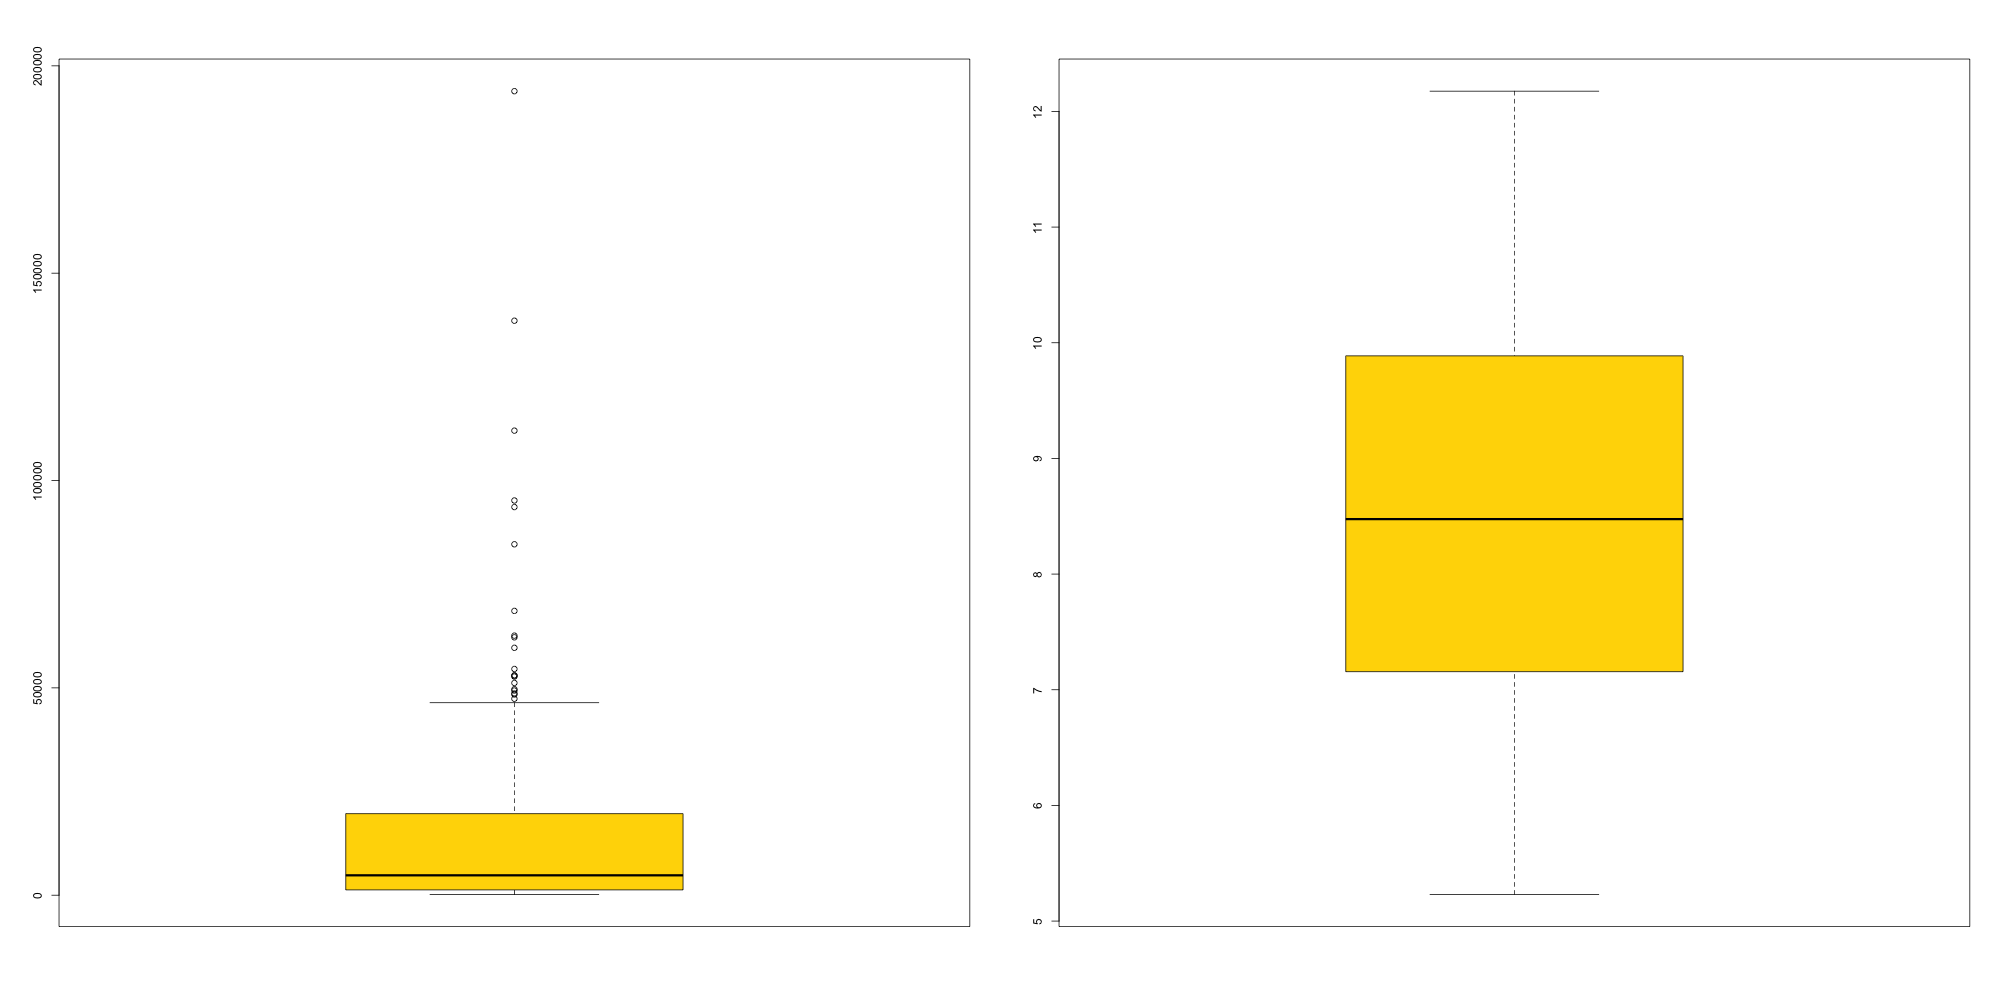
\includegraphics[width=\textwidth]{images/gdp_transform}
  \caption{\label{gdp_transform}Log GDP per capita is more normal than its unlogged counterpart.}
\end{figure}

%\begin{figure}[!ht] \centering \includegraphics[scale=0.5]{images/gdp_per_capita_heat_map.jpg} \caption{\label{gdp_per_capita_heat_map}Our response had near-universal coverage.} \end{figure}









% % % % % % % % % % % % % % % % % % % % % %
% % % % % % % % % % % % % % % % % % % % % %
% % % % % % % % % % % % % % % % % % % % % %
% % % % % % % % % % % % % % % % % % % % % %
% % % % % % % % % % % % % % % % % % % % % %
% % % % % % % % % % % % % % % % % % % % % %
% % % % % % % % % % % % % % % % % % % % % %
% % % % % % % % % % % % % % % % % % % % % %
% % % % % % % % % % % % % % % % % % % % % %
\section{Climate Change Model}
\label{sec:model_climate}

% % % % % % % % % % %
% % % % % % % % % % %
% % % % % % % % % % %
\subsection{Indicators}
How do climate-related indicators affect a country's wealth? To answer this, we look at pollution and energy consumption. Intuitively, there is a correlation between those two: the more energy a country consumes, the more it pollutes. We proceed with caution, wary of multicollinearity.

For our pollution metrics, we choose emissions (measured in kilotons) consisting of three basic chemical compounds: nitrous oxide, carbon dioxide, and methane. Nitrous oxide emissions result from agricultural biomass burning, industrial activity, and livestock management. Carbon dioxide results from burning fossil fuels. Methane results from agriculture and industry.

Our proxies for energy consumption consist of electric consumption per capita (in kilowatt-hours) and the percentage of total roads that are paved. The former measures the production of power plants (minus transportation costs), while the latter might directly account for those transportation costs: that is, a larger network of paved roads may reduce the time it takes to transport goods and thus energy consumption.

When we run scatterplots of each of the pollution metrics against the response, none resemble anything close to a linear relationship. When we apply a log transformation to each pollution metric, however, all of them exhibit linearity. This correction is illustrated in Figure~\ref{climate_model_scatter_pollution}.

\begin{figure*}[!ht]
  \centering
  \includegraphics[width=0.8\textwidth]{images/climate_model_scatter_pollution}
  \caption{\label{climate_model_scatter_pollution}Left to right: CO2, methane, nitrous. Log transformations on bottom row.}
\end{figure*}

Next we run scatterplots of log GDP per capita versus each our proxies for energy consumption, as shown in the top row of Figure~\ref{climate_model_scatter_elec_roads}. Immediately we see two problems. First, electricity consumption versus log GDP per capita does not exhibit linearity. Second, the number of data points for the paved roads indicator is minimal. A log transformation on each indicator is shown in the bottom row. The log of electricity consumption exhibits a more linear relationship with the response. However, paved roads still has just as few data points.

\begin{figure*}[!ht]
  \centering
  \includegraphics[width=0.6\textwidth]{images/climate_model_scatter_elec_roads}
  \caption{\label{climate_model_scatter_elec_roads}Left to right: electricity consumption, paved roads. Log transformations on bottom row.}
\end{figure*}

% % % % % % % % % % %
% % % % % % % % % % %
% % % % % % % % % % %
\subsection{Regression}
Table~\ref{climate_model_regressions} shows our variations of the climate model.
First, we run the full model that includes every indicator.
Of these, the log of electricity consumption is the only one to show up as significant.
We see a positive correlation: the more energy power plants consume in a country, the higher that country's log per-capita GDP will be.
Specifically, for the models 1 and 3, a 1\% increase in electricity consumption is associated with $0.97$\% increase in GDP per capita, give or take one basis point.

\newgeometry{margin=1cm} % modify this if you need even more space
\begin{landscape}
\begin{table}[!htbp] \centering 
  \caption{$N$ increases when we remove paved roads.}
  \label{climate_model_regressions} 
\begin{tabular}{@{\extracolsep{5pt}}lcccc} 
\\[-1.8ex]\hline 
\hline \\[-1.8ex] 
 & \multicolumn{4}{c}{\textit{Dependent variable:}} \\ 
\cline{2-5} 
\\[-1.8ex] & \multicolumn{4}{c}{log.GDP.per.capita} \\ 
\\[-1.8ex] & (1) & (2) & (3) & (4)\\ 
\hline \\[-1.8ex] 
 paved.roads & 0.003 & 0.001 & $-$0.001 &  \\ 
  & (0.003) & (0.003) & (0.016) &  \\ 
  & & & & \\ 
 log.electricity.consumption & 0.984$^{***}$ & 0.411 & 0.962$^{***}$ & 0.291 \\ 
  & (0.098) & (0.313) & (0.071) & (0.212) \\ 
  & & & & \\ 
 paved.roads:log.co2 &  &  & 0.0003 &  \\ 
  &  &  & (0.002) &  \\ 
  & & & & \\ 
 log.co2 & $-$0.049 & $-$0.454$^{*}$ & $-$0.017 & $-$0.455$^{***}$ \\ 
  & (0.127) & (0.257) & (0.106) & (0.172) \\ 
  & & & & \\ 
 log.nitrous & 0.100 &  &  &  \\ 
  & (0.122) &  &  &  \\ 
  & & & & \\ 
 log.methane & $-$0.066 &  &  &  \\ 
  & (0.165) &  &  &  \\ 
  & & & & \\ 
 log.electricity.consumption:log.co2 &  & 0.058$^{*}$ &  & 0.061$^{***}$ \\ 
  &  & (0.032) &  & (0.022) \\ 
  & & & & \\ 
 Constant & 1.465$^{*}$ & 5.736$^{**}$ & 1.557 & 6.433$^{***}$ \\ 
  & (0.865) & (2.491) & (1.105) & (1.626) \\ 
  & & & & \\ 
\hline \\[-1.8ex] 
Observations & 58 & 59 & 59 & 132 \\ 
R$^{2}$ & 0.842 & 0.840 & 0.831 & 0.806 \\ 
Adjusted R$^{2}$ & 0.827 & 0.829 & 0.818 & 0.802 \\ 
Residual Std. Error & 0.591 (df = 52) & 0.584 (df = 54) & 0.601 (df = 54) & 0.668 (df = 128) \\ 
F Statistic & 55.543$^{***}$ (df = 5; 52) & 71.067$^{***}$ (df = 4; 54) & 66.321$^{***}$ (df = 4; 54) & 177.733$^{***}$ (df = 3; 128) \\ 
\hline 
\hline \\[-1.8ex] 
\textit{Note:}  & \multicolumn{4}{r}{$^{*}$p$<$0.1; $^{**}$p$<$0.05; $^{***}$p$<$0.01} \\ 
\end{tabular} 
\end{table} 
\end{landscape}
\restoregeometry
\doublespacing

However, Model 4 tells a different story.
We remove the paved roads indicator -- as it is causing too many values to be deleted -- and regress on the interaction between log CO2 and log electricity consumption.
We find that the log of electricity consumption is no longer significant.
Instead, log CO2 and the interaction term are significant.

% % % % % % % % % % %
% % % % % % % % % % %
% % % % % % % % % % %
\subsection{Condition Checking}
As with any linear regression model, we provide exploratory analysis of our assumptions: linearity, independence, zero mean, constant variance, and normality.

We confirm (1) linearity above with scatterplots, (2) zero error mean by our use of ordinary least squares linear regression, and (3) independence by the way data points were collected -- that is, measuring a nation's statistics does not effect the statistics of it or any other nation. We apply these assumptions to the other three models.

Figure~\ref{climate_model_conditions} provides a way for us to assess whether our model violates our assumptions of equal variance and normal errors. On the left, we see a scatterplot of residuals versus fitted values, which shows that the model is fairly homoskedastic. On the right, we see the errors are not quite normal, as there is a long left tail. For future work, we might try nonparametric tests, as they do not require a normal error distribution.


\begin{figure*}[!ht]
  \centering
  \includegraphics[width=\textwidth]{images/climate_model_conditions}
  \caption{\label{climate_model_conditions}Residuals vs fitted and Q-Q plot}
\end{figure*}












% % % % % % % % % % % % % % % % % % % % % %
% % % % % % % % % % % % % % % % % % % % % %
% % % % % % % % % % % % % % % % % % % % % %
% % % % % % % % % % % % % % % % % % % % % %
% % % % % % % % % % % % % % % % % % % % % %
% % % % % % % % % % % % % % % % % % % % % %
% % % % % % % % % % % % % % % % % % % % % %
% % % % % % % % % % % % % % % % % % % % % %
% % % % % % % % % % % % % % % % % % % % % %
\section{Cities Model}
\label{sec:model_urban}

% % % % % % % % % % %
% % % % % % % % % % %
% % % % % % % % % % %
\subsection{Indicators}
How well does a country's urban environment explain its wealth? To answer this, we look at the size of a country's urban environment, as well as the welfare of that environment.
For size, we use the percentage of population living in urban environments.
For welfare, we use the percentage of the urban population with access to clean water. Figure~\ref{urban_model_scatter_pop_water} shows scatterplots of log GDP per capita against our \emph{population} and \emph{water} indicators.

\begin{figure*}[!ht]
  \centering
  \includegraphics[width=0.8\textwidth]{images/urban_model_scatter_pop_water}
  \caption{\label{urban_model_scatter_pop_water}Left to right: Population, water.}
\end{figure*}

We lack a linear relationship between the response and the percentage of urban population with access to water. We tried to remedy this defect with several transformations, but to no avail. Consequently, we replace our urban welfare predictor with the percentage of the urban population with access to sanitation, which primarily entails access to latrines. This new indicator exhibited a much more linear relationship with log GDP per capita, as seen in Figure~\ref{urban_model_scatter_san}.

\begin{figure*}[!ht]
  \centering
  \includegraphics[width=0.4\textwidth]{images/urban_model_scatter_san}
  \caption{\label{urban_model_scatter_san}Access to sanitation is a better proxy for urban welfare than access to water.}
\end{figure*}

% % % % % % % % % % %
% % % % % % % % % % %
% % % % % % % % % % %
\subsection{Regression}

Table~\ref{urban_model_regressions} shows the regressions of various phases of our urban model.
The first model includes our size metric (urban population) as well as both of our proxies for urban welfare (urban sanitation and urban water).
Model 2 regresses log GDP per capita on urban population and urban water, whereas Model 3 regresses on urban population and urban sanitation.

%\newgeometry{margin=1cm} % modify this if you need even more space
%\begin{landscape}
\begin{table}[!htbp] \centering 
  \caption{We drop urban water in the final model, due to its lack of linearity.}
  \label{urban_model_regressions} 
\begin{tabular}{@{\extracolsep{5pt}}lccc} 
\\[-1.8ex]\hline 
\hline \\[-1.8ex] 
 & \multicolumn{3}{c}{\textit{Dependent variable:}} \\ 
\cline{2-4} 
\\[-1.8ex] & \multicolumn{3}{c}{log.GDP.per.capita} \\ 
\\[-1.8ex] & (1) & (2) & (3)\\ 
\hline \\[-1.8ex] 
 urban.population & 0.032$^{***}$ & 0.042$^{***}$ & 0.033$^{***}$ \\ 
  & (0.003) & (0.003) & (0.003) \\ 
  & & & \\ 
 urban.sanitation & 0.028$^{***}$ &  & 0.032$^{***}$ \\ 
  & (0.003) &  & (0.003) \\ 
  & & & \\ 
 urban.water & 0.022$^{**}$ & 0.061$^{***}$ &  \\ 
  & (0.009) & (0.010) &  \\ 
  & & & \\ 
 Constant & 2.449$^{***}$ & 0.373 & 4.141$^{***}$ \\ 
  & (0.752) & (0.841) & (0.199) \\ 
  & & & \\ 
\hline \\[-1.8ex] 
Observations & 179 & 183 & 181 \\ 
R$^{2}$ & 0.761 & 0.664 & 0.756 \\ 
Adjusted R$^{2}$ & 0.757 & 0.661 & 0.753 \\ 
Residual Std. Error & 0.781 (df = 175) & 0.922 (df = 180) & 0.787 (df = 178) \\ 
F Statistic & 186.043$^{***}$ (df = 3; 175) & 178.061$^{***}$ (df = 2; 180) & 275.727$^{***}$ (df = 2; 178) \\ 
\hline 
\hline \\[-1.8ex] 
\textit{Note:}  & \multicolumn{3}{r}{$^{*}$p$<$0.1; $^{**}$p$<$0.05; $^{***}$p$<$0.01} \\ 
\end{tabular} 
\end{table}
\end{landscape}
%\restoregeometry
%\doublespacing

Every indicators in each of the models appears significant, but we should expect the highest $R^2$ from the last model, since its welfare proxy (\emph{urban sanitation}) bears a much more linear relationship with the response than the other welfare proxy (\emph{urban water}). Indeed, the $R^2$ of Model 2 is $0.66$, whereas the $R^2$ of Model 3 is $0.75$.


% % % % % % % % % % %
% % % % % % % % % % %
% % % % % % % % % % %
\subsection{Condition Checking}
Figure~\ref{urban_model_conditions} allows us to assess our model condition's of equal variance and normal errors. The scatterplot of residuals versus fitted values shows roughly equal variance for all fitted values. The Q-Q plot, on the other hand, is not as promising, as we see a slightly long left tail. If we believe the lack of normality in the errors is a concern, we could perform nonparametric tests, which punt on assumptions about the error distribution.

\begin{figure}[!ht]
  \centering
  \includegraphics[width=0.8\textwidth]{images/urban_model_conditions}
  \caption{\label{urban_model_conditions}The urban model shows equal variance and (almost) normal errors.}
\end{figure}







% % % % % % % % % % % % % % % % % % % % % %
% % % % % % % % % % % % % % % % % % % % % %
% % % % % % % % % % % % % % % % % % % % % %
% % % % % % % % % % % % % % % % % % % % % %
% % % % % % % % % % % % % % % % % % % % % %
% % % % % % % % % % % % % % % % % % % % % %
% % % % % % % % % % % % % % % % % % % % % %
% % % % % % % % % % % % % % % % % % % % % %
% % % % % % % % % % % % % % % % % % % % % %
\section{Computers Model}
\label{sec:model_tech}

% % % % % % % % % % %
% % % % % % % % % % %
% % % % % % % % % % %
\subsection{Indicators}
How well does a country's level of technology explain its wealth? We examine three indicators: the number of scientific journals and articles produced by a nation, the percent of GDP that goes into research and development (R\&D), and the percentage of manufactured exports that are deemed ``high-tech.'' It is worth noting that each of these explanatory variables may be highly correlated with each other. In other words, the more a country invests in R\&D, the more scientific journals it will produce, and vice versa.
% TODO correlation matrix

\begin{figure}[!ht]
  \centering
  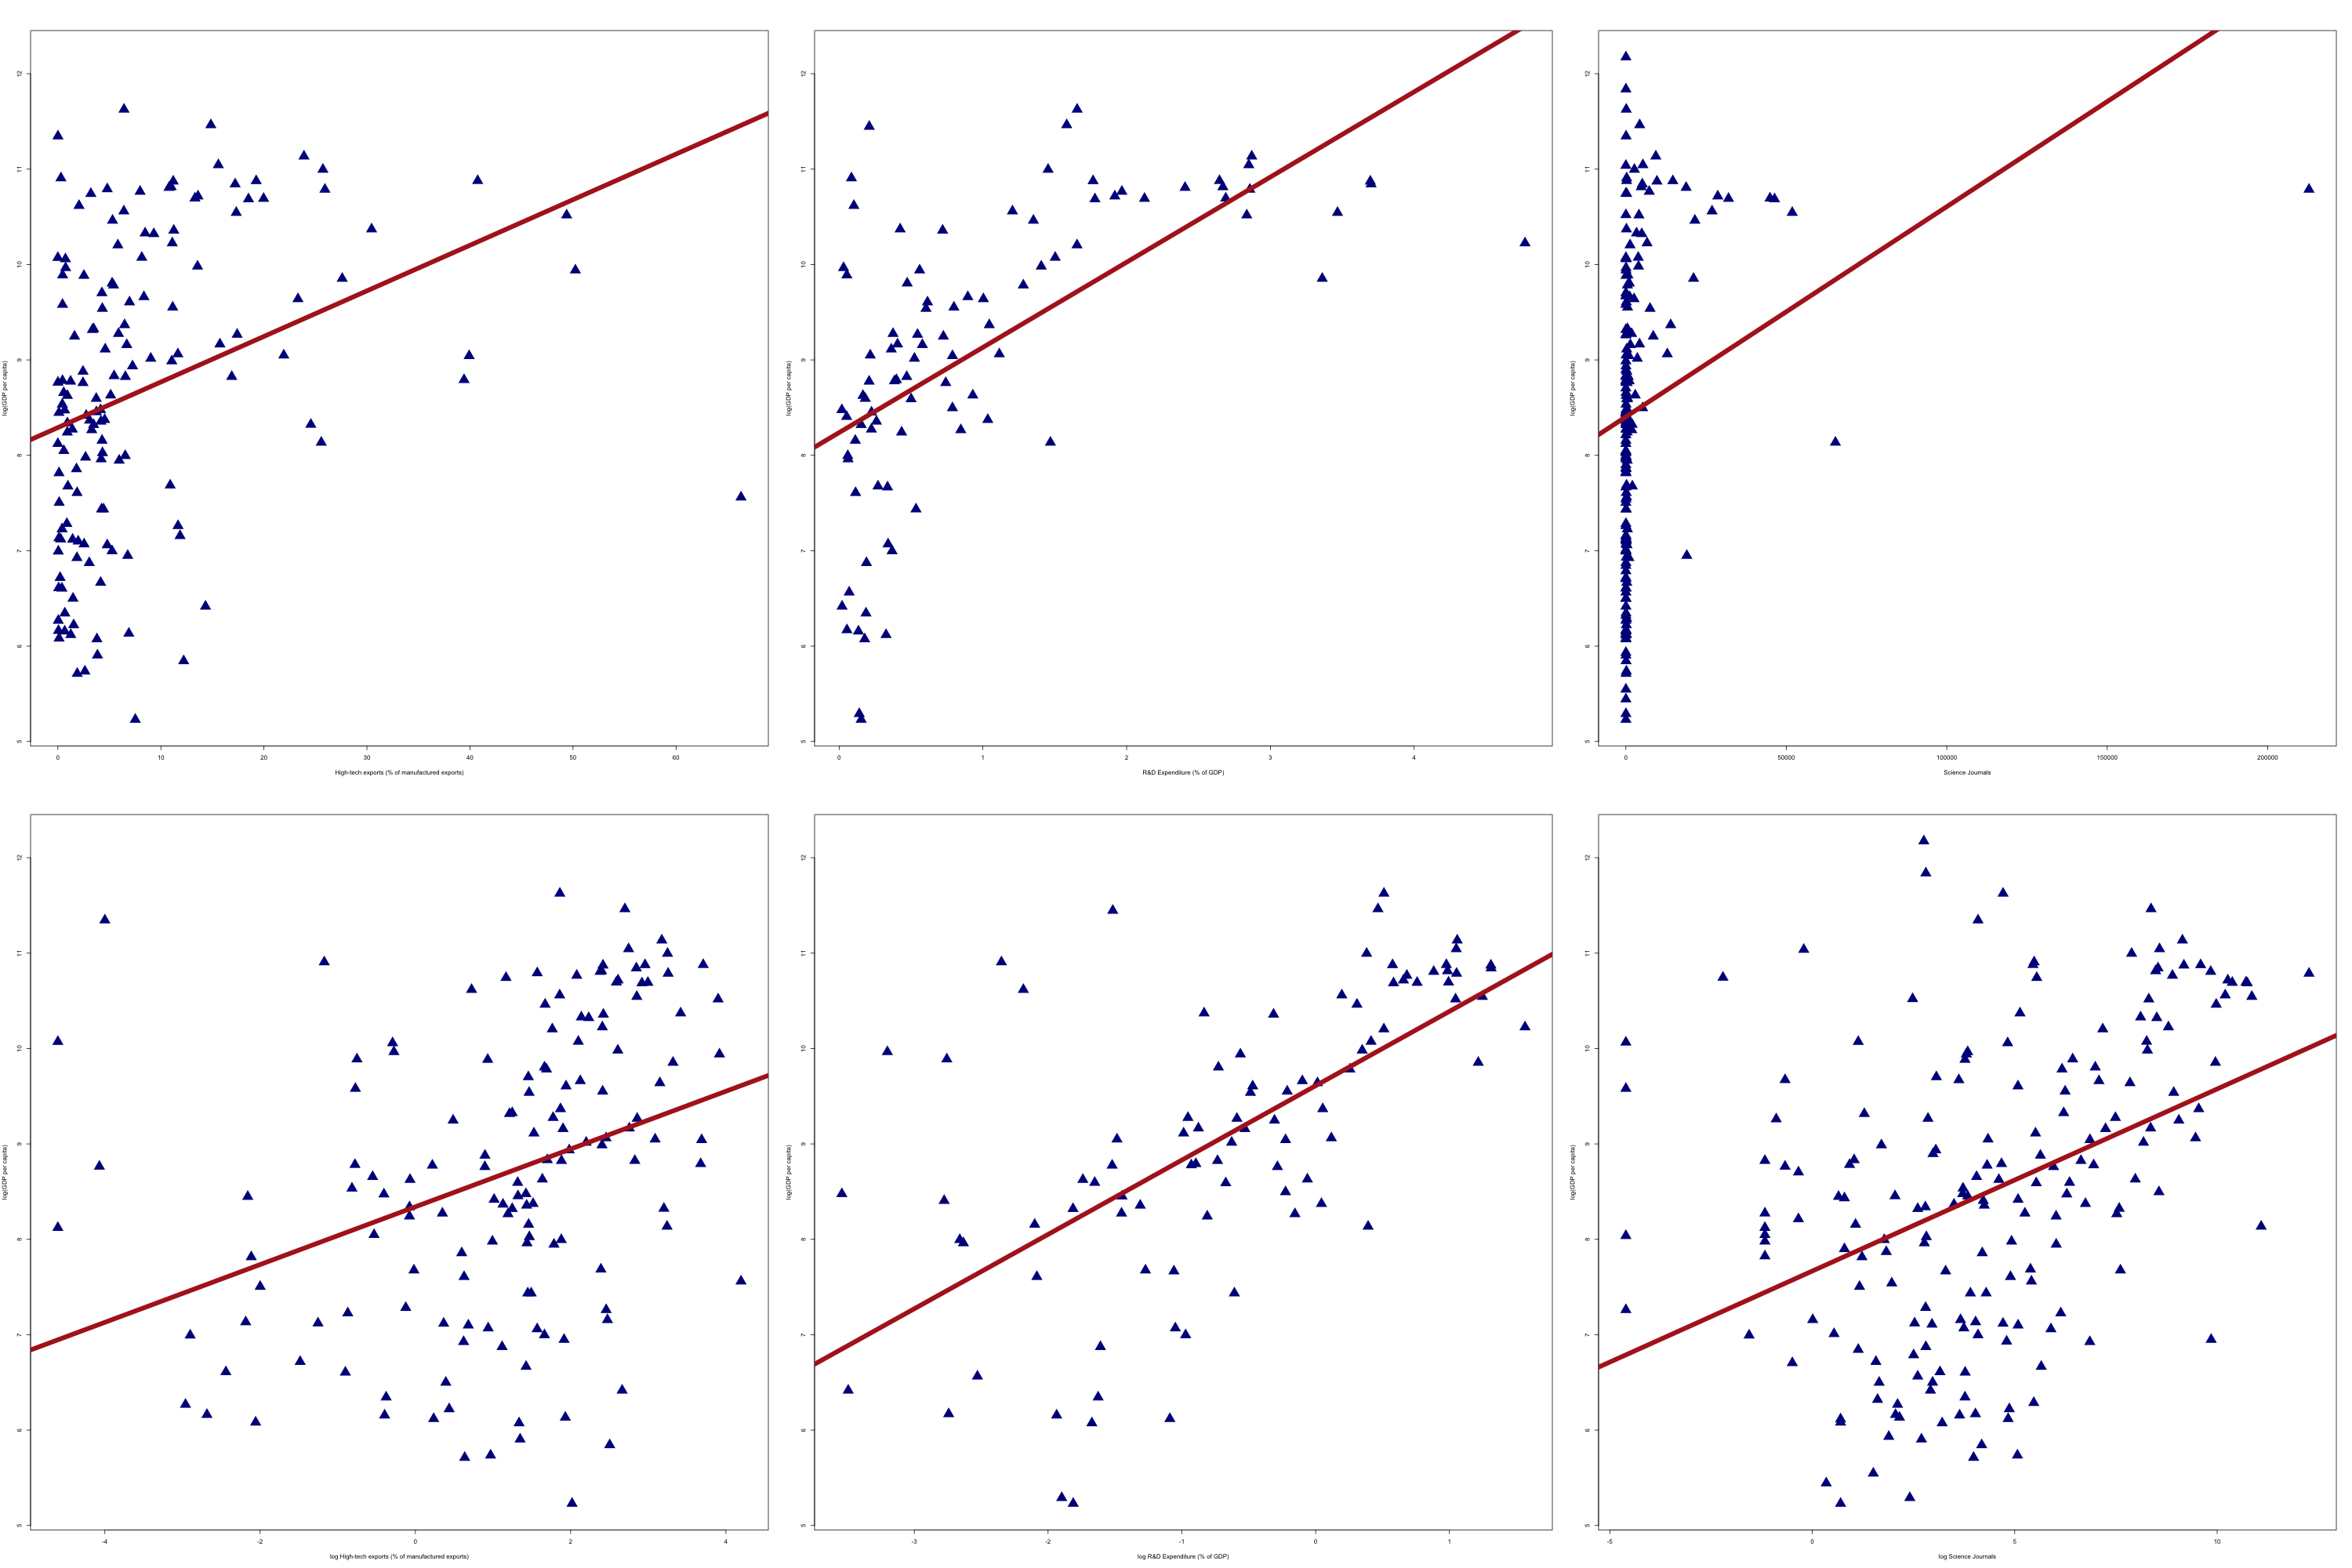
\includegraphics[width=0.8\textwidth]{images/science_model_scatter}
  \caption{\label{science_model_scatter}Left to right: exports, R\&D, journals. Logs on bottom.}
\end{figure}

% % % % % % % % % % %
% % % % % % % % % % %
% % % % % % % % % % %
\subsection{Regression}

Once we apply log transformations to each of our three indicators, we see strong linear relationships, shown in Figure~\ref{science_model_scatter}.

Table~\ref{science_model_regressions} shows various forms of our science and technology model. We use the logarithms of our World Bank indicators, as they are stronger predictors of log GDP per capita.

In addition, we include every possible interaction term for two reasons.
First, we do so because we can afford to. With only $K=3$ explanatory variables, we can show all $6 = K(K-1)/2$ pairwise combinations. 
Second, and more importantly, we suspect that the effect of one explanatory variable on log GDP per capita depends on the level of another covariate. For instance, research may have less impact on GDP for lower levels of high-tech exports. This is intuitive since, in our model, research is only as good as the fruits borne by it. In short, we justify our use of interaction terms with the following question: What's the point of science journals and R\&D if you can't make things?

Table~\ref{science_model_regressions} answers precisely that question. Indeed, there is no ``point'' -- in the sense of output and GDP -- to the science community if it doesn't produce anything. We know this because
$\ln(\mathrm{research}) \times \ln(\mathrm{high.tech})$ and
$\ln(\mathrm{high.tech}) \times \ln(\mathrm{journals})$
are significant, but 
$\ln(\mathrm{research}) \times \ln(\mathrm{journals})$ is not.

\newgeometry{margin=1cm} % modify this if you need even more space
\begin{landscape}
\small
\begin{table}[!htbp] \centering 
  \caption{Taking out \emph{research} drastically increases the number of observations.}
  \label{science_model_regressions} 
\begin{tabular}{@{\extracolsep{5pt}}lccccc} 
\\[-1.8ex]\hline 
\hline \\[-1.8ex] 
 & \multicolumn{5}{c}{\textit{Dependent variable:}} \\ 
\cline{2-6} 
\\[-1.8ex] & \multicolumn{5}{c}{log.GDP.per.capita} \\ 
\\[-1.8ex] & (1) & (2) & (3) & (4) & (5)\\ 
\hline \\[-1.8ex] 
 log.research & 0.324$^{*}$ & 0.576$^{**}$ & $-$0.076 &  & $-$0.758$^{**}$ \\ 
  & (0.178) & (0.277) & (0.225) &  & (0.339) \\ 
  & & & & & \\ 
 log.journals & 0.212$^{***}$ & 0.206$^{***}$ &  & 0.108$^{**}$ & 0.661$^{***}$ \\ 
  & (0.071) & (0.070) &  & (0.052) & (0.151) \\ 
  & & & & & \\ 
 log.high.tech:log.journals &  &  &  & 0.066$^{***}$ & $-$0.237$^{***}$ \\ 
  &  &  &  & (0.019) & (0.063) \\ 
  & & & & & \\ 
 log.high.tech & 0.179 &  & 0.512$^{***}$ & $-$0.102 & 2.115$^{***}$ \\ 
  & (0.129) &  & (0.161) & (0.091) & (0.429) \\ 
  & & & & & \\ 
 log.research:log.journals &  & $-$0.018 &  &  & 0.021 \\ 
  &  & (0.041) &  &  & (0.045) \\ 
  & & & & & \\ 
 log.research:log.high.tech &  &  & 0.367$^{***}$ &  & 0.544$^{***}$ \\ 
  &  &  & (0.093) &  & (0.098) \\ 
  & & & & & \\ 
 Constant & 7.638$^{***}$ & 8.054$^{***}$ & 8.301$^{***}$ & 7.620$^{***}$ & 3.785$^{***}$ \\ 
  & (0.652) & (0.559) & (0.408) & (0.216) & (1.057) \\ 
  & & & & & \\ 
\hline \\[-1.8ex] 
Observations & 79 & 88 & 81 & 143 & 79 \\ 
R$^{2}$ & 0.499 & 0.521 & 0.504 & 0.326 & 0.655 \\ 
Adjusted R$^{2}$ & 0.479 & 0.504 & 0.484 & 0.311 & 0.626 \\ 
Residual Std. Error & 1.050 (df = 75) & 1.067 (df = 84) & 1.042 (df = 77) & 1.282 (df = 139) & 0.890 (df = 72) \\ 
F Statistic & 24.942$^{***}$ (df = 3; 75) & 30.418$^{***}$ (df = 3; 84) & 26.041$^{***}$ (df = 3; 77) & 22.394$^{***}$ (df = 3; 139) & 22.737$^{***}$ (df = 6; 72) \\ 
\hline 
\hline \\[-1.8ex] 
\textit{Note:}  & \multicolumn{5}{r}{$^{*}$p$<$0.1; $^{**}$p$<$0.05; $^{***}$p$<$0.01} \\ 
\end{tabular} 
\end{table} 
\end{landscape}
\restoregeometry
\doublespacing


% % % % % % % % % % %
% % % % % % % % % % %
% % % % % % % % % % %
\subsection{Condition Checking}

Figure~\ref{science_model_conditions} shows the regression conditions for the following model:
\begin{align*}
\ln(\textrm{GDP per capita}) = \beta_0 &+
\beta_1 \cdot \ln(\textrm{research}) +
\beta_2 \cdot \ln(\textrm{exports}) +
\beta_3 \cdot \ln(\textrm{journals}) + \\
&\beta_4 \cdot \ln(\textrm{research}) \times \ln(\textrm{journals}) + \\
&\beta_5 \cdot \ln(\textrm{exports}) \times \ln(\textrm{research}) + \\
&\beta_6 \cdot \ln(\textrm{exports}) \times \ln(\textrm{journals})
\end{align*}
From the plot of residuals versus fitted values, we can glean that there is fairly equal variance.
From the Q-Q plot, we see that the errors are roughly normal, with some deviation on the left tail.

\begin{figure}[!ht]
  \centering
  \includegraphics[width=0.7\textwidth]{images/science_model_conditions}
  \caption{\label{science_model_conditions}Left to right: Residuals vs fitted values, Q-Q plot.}
\end{figure}


% % % % % % % % % % % % % % % % % % % % % %
% % % % % % % % % % % % % % % % % % % % % %
% % % % % % % % % % % % % % % % % % % % % %
% % % % % % % % % % % % % % % % % % % % % %
% % % % % % % % % % % % % % % % % % % % % %
% % % % % % % % % % % % % % % % % % % % % %
% % % % % % % % % % % % % % % % % % % % % %
% % % % % % % % % % % % % % % % % % % % % %
% % % % % % % % % % % % % % % % % % % % % %
\section{Social Development Model}
\label{sec:model_social}

% % % % % % % % % % %
% % % % % % % % % % %
% % % % % % % % % % %
\subsection{Indicators}
How does a country's level of social development affect its output, and more importantly, its GDP per capita?
We look at four primary indicators: the unemployment rate for children ages 7-14, the life expectancy at birth (in years) for males, the refugee population, and the literacy rate for adults aged 15 and above.
These indicators measure a country's economic, health, political, and educational institutions, respectively.
Intuition tells us they are positively correlated with national output.
That is, we expect GDP per capita to rise with lower unemployment rates, higher life expectancy, a lower refugee population, and higher levels of education.

% % % % % % % % % % %
% % % % % % % % % % %
% % % % % % % % % % %
\subsection{Regression}
Table~\ref{social_development_model_regressions} shows our social development model.
Model 1 and model 2 simply show that child labor and literacy, though significant, do not have enough observations.
For this reason, we focus on model 3, which shows that $\ln(\mathrm{life.expect})$ and $\ln(\mathrm{refugees})$ have an extremely statistically significant effect on $ln(\mathrm{GDP.per.capita})$.

\begin{table}[!htbp] \centering 
  \caption{Sufficently large $n$ acquired from removing child labor and literacy.}
  \label{social_development_model_regressions} 
\begin{tabular}{@{\extracolsep{5pt}}lccc} 
\\[-1.8ex]\hline 
\hline \\[-1.8ex] 
 & \multicolumn{3}{c}{\textit{Dependent variable:}} \\ 
\cline{2-4} 
\\[-1.8ex] & \multicolumn{3}{c}{log.GDP.per.capita} \\ 
\\[-1.8ex] & (1) & (2) & (3)\\ 
\hline \\[-1.8ex] 
 log.child.labor & $-$0.968$^{**}$ &  &  \\ 
  & (0.314) &  &  \\ 
  & & & \\ 
 log.literacy &  & 3.234$^{**}$ &  \\ 
  &  & (1.387) &  \\ 
  & & & \\ 
 log.life.expect &  &  & 6.981$^{***}$ \\ 
  &  &  & (0.534) \\ 
  & & & \\ 
 log.refugees &  &  & $-$0.136$^{***}$ \\ 
  &  &  & (0.023) \\ 
  & & & \\ 
 Constant & 10.128$^{***}$ & $-$5.968 & $-$19.888$^{***}$ \\ 
  & (0.934) & (6.156) & (2.303) \\ 
  & & & \\ 
\hline \\[-1.8ex] 
Observations & 12 & 25 & 180 \\ 
R$^{2}$ & 0.487 & 0.191 & 0.633 \\ 
Adjusted R$^{2}$ & 0.436 & 0.156 & 0.628 \\ 
Residual Std. Error & 0.951 (df = 10) & 1.278 (df = 23) & 0.968 (df = 177) \\ 
F Statistic & 9.496$^{**}$ (df = 1; 10) & 5.438$^{**}$ (df = 1; 23) & 152.374$^{***}$ (df = 2; 177) \\ 
\hline 
\hline \\[-1.8ex] 
\textit{Note:}  & \multicolumn{3}{r}{$^{*}$p$<$0.1; $^{**}$p$<$0.05; $^{***}$p$<$0.01} \\ 
\end{tabular} 
\end{table} 

% % % % % % % % % % %
% % % % % % % % % % %
% % % % % % % % % % %
\subsection{Condition Checking}
The conditions of model 3 are depicted in Figure~\ref{social_model_conditions}.
From the plot of residuals versus fitted values, we see that the variance is not fan-shaped, but it is also far from ideal.
From the model's Q-Q plot, we see that the error distribution is far from normal, since both tails are long.
Thus, our social development model may require a nonparametric test.

\begin{figure}[!ht]
  \centering
  \includegraphics[width=0.7\textwidth]{images/social_model_conditions}
  \caption{\label{social_model_conditions}Left to right: Residuals vs fitted values, Q-Q plot.}
\end{figure}



















% % % % % % % % % % % % % % % % % % % % % %
% % % % % % % % % % % % % % % % % % % % % %
% % % % % % % % % % % % % % % % % % % % % %
% % % % % % % % % % % % % % % % % % % % % %
% % % % % % % % % % % % % % % % % % % % % %
% % % % % % % % % % % % % % % % % % % % % %
% % % % % % % % % % % % % % % % % % % % % %
% % % % % % % % % % % % % % % % % % % % % %
% % % % % % % % % % % % % % % % % % % % % %
\section{Conclusion}
\label{sec:conclusion}
We provide four core models that explain the log of GDP per capita.
Each model has very significant indicators and high $R^2$.
More importantly, these models are more relatable and more interesting to the layman than Keynesian theory.
That is, they offer a fresh explanation for why some nations are wealthier by regressing on more perceptible variables, such as a country's general levels of pollution, urbanization, innovation, and education.

However, there may be an inherent limitation to our regressions: reverse causality.
In each model we try to explain the effect of $x$ on $y$, when in reality it could be that $y$ affects $x$. For instance, a country's GDP per capita may be what allows it to invest more in research and technology.

Even if $y$ does not directly cause $x$, it may affect $x$ through another lurking variable. We must think about what affects the indicators we use. First, we do not account for a nation's institutions, even though they have a huge impact on just about everything. Wealthier nations can afford to have strengthen their legal and political institutions. As a result, regulations on pollution or on child labor may be more stringent.

Another limitation might be multicollinearity between two or more indicators in a regression. Often, two explanatory variables are literally proxies for the same thing, as was the case with methane emissions and nitrous emissions; they both proxy for pollution. Sometimes one covariate affects another. This occurred in the climate change model, since higher energy consumption almost certainly increases pollution. Additionally, we speculate that it may have occurred in the social development model: higher literacy rates may rise with productivity, which may eliminate the need for children workers.

In the case of multicollinearity, regressions can fail. In the case of reverse causality, covariates can be correlated with the error terms. There are several methods to fix the problem of biased and inconsistent estimates -- such as instrumental variables, decision tree predictor selection, stepwise regressions -- but they are all beyond the scope of introductory statistics.

By far, the easiest way to deal with bias is to manually remove one or more of the explanatory variables. Collinear covariates can be weeded on mere suspicion, or based on the variance inflation factor (VIF). For instance, if the VIF for \emph{nitrous emissions} is 9, this means $SE(\beta_{\textrm{nitrous emissions}})$ is $\sqrt{9} = 3$ times as large as it would be if \emph{nitrous emissions} were not correlated with any other predictors.

Our models are not without their flaws, but we have provided a preliminary investigation into what is required to explain a country's per capita wealth in a robust and unbiased way.


\endnotetext[1]{For modularity, we built a script that created a data frame for each year of data downloaded, and then recast each frame from wide to long format.}

\theendnotes

\end{document}
